\documentclass[a4paper, 11pt]{article}
\usepackage{comment}
\usepackage{lipsum} 
\usepackage{fullpage} %cambiar margen
\usepackage[a4paper, total={7in, 10in}]{geometry}

\usepackage{amssymb,amsthm} 
\usepackage{amsmath}
\newtheorem{theorem}{Theorem}
\newtheorem{corollary}{Corollary}
\usepackage{graphicx}
\usepackage{tikz}
\usetikzlibrary{arrows}
\usepackage{verbatim}
%\usepackage[numbered]{mcode}
\usepackage{float}
\usepackage{tikz}
\usetikzlibrary{shapes,arrows}
\usetikzlibrary{arrows,calc,positioning}
\usepackage{mathpazo} %tipo de letra 
\usepackage[utf8]{inputenc} %codificación
\usepackage[T1]{fontenc} %digitación de tildes y ñ
\usepackage[spanish]{babel} %paquete de soporte español

\tikzset{
	block/.style = {draw, rectangle,
		minimum height=1cm,
		minimum width=1.5cm},
	input/.style = {coordinate,node distance=1cm},
	output/.style = {coordinate,node distance=4cm},
	arrow/.style={draw, -latex,node distance=2cm},
	pinstyle/.style = {pin edge={latex-, black,node distance=2cm}},
	sum/.style = {draw, circle, node distance=1cm},
}
\usepackage{xcolor}
\usepackage{mdframed}
\usepackage[shortlabels]{enumitem}
\usepackage{indentfirst}
\usepackage{hyperref}

\usepackage{listings}
\lstset{literate=
  {á}{{\'a}}1
  {é}{{\'e}}1
  {í}{{\'i}}1
  {ó}{{\'o}}1
  {ú}{{\'u}}1
  {Á}{{\'A}}1
  {É}{{\'E}}1
  {Í}{{\'I}}1
  {Ó}{{\'O}}1
  {Ú}{{\'U}}1
  {ñ}{{\~n}}1
  {ü}{{\"u}}1
  {Ü}{{\"U}}1
}

\lstdefinestyle{customc}{
  belowcaptionskip=1\baselineskip,
  breaklines=true,
  frame=L,
  xleftmargin=\parindent,
  language=Python,
  showstringspaces=false,
  basicstyle=\footnotesize\ttfamily,
  keywordstyle=\bfseries\color{green!40!black},
  commentstyle=\itshape\color{purple!40!black},
  identifierstyle=\color{blue},
  stringstyle=\color{orange},
}

\lstdefinestyle{customasm}{
  belowcaptionskip=1\baselineskip,
  frame=L,
  xleftmargin=\parindent,
  language=[x86masm]Assembler,
  basicstyle=\footnotesize\ttfamily,
  commentstyle=\itshape\color{purple!40!black},
}

\lstset{escapechar=@,style=customc}



\renewcommand{\thesubsection}{\thesection.\alph{subsection}}

\newenvironment{problem}[2][Ejercicio]
{ \begin{mdframed}[backgroundcolor= red!50] \textbf{#1 #2} \\}
	{  \end{mdframed}}

% Define solution environment
\newenvironment{solution}
{\textcolor{blue}{\textbf{\textit{Solución:\\\noindent}}}}


\renewcommand{\qed}{\quad\qedsymbol}

% \\	
\begin{document}
	\noindent
	%%%%%%%%%%%%%%%%%%%%%%%%%%%%%%%%%%%%
	
	\begin{minipage}[b][1.2cm][t]{0.8\textwidth}
		\large\textbf{César Isaí García Cornejo} \hfill \textbf{A systematic review of Python...}  \\
		cesar.cornejo@cimat.mx \hfill \\
		\normalsize Series de Tiempo \hfill Semestre 3\\
	\end{minipage}
	
	\hspace{14.4cm}
	\begin{minipage}[b][0.03cm][t]{0.12\linewidth}
		
		\vspace{-2.2cm}
		%%%La Ruta depeendera de donde este alojado el main y la imagen
		
\includegraphics[scale=0.3]{Figures/EscudoCimat.png}
	\end{minipage}
	
	\noindent\rule{7in}{2.8pt}
	
	%%%%%%%%%%%%%%%%%%%%%
	%%%%%%%%%%%%%%%%%%%%%%%%%%%%%%%%%%%%%%%%%%%%%%%%%%%%%%%%%%%%%%%%%%%%%%%%%%%%%%%%%%%%%%%%%%%%%%%%%%%%%%%%%%%%%%%%%%%
	% Problem 1
	%%%%%%%%%%%%%%%%%%%%%%%%%%%%%%%%%%%%%%%%%%%%%%%%%%%%%%%%%%%%%%%%%%%%%%%%%%%%%%%%%%%%%%%%%%%%%%%%%%%%%%%%%%%%%%%%%%%%%%%%%%%%%%%%%%%%%%%%
	\setlength{\parskip}{\medskipamount}
	\setlength{\parindent}{0pt}
 %///////////////////////////////////////////////////
\section*{Abstract}

El articulo presenta una comparación de varias paqueterías de Python para series de tiempo. Su objetivo es presentar un panorama de diferentes cometidos y métodos implementados, esto incluye documentación, dependencias y sus comunidades. Fueron análizados 40 paqueterías, y las clasificaron de acuerdo a sus labores implementadas, los métodos para el preprocesamiento y licencias. Entre todos los objetivos, se encontro que el más frecuente son los pronosticos. La mitas de las paqueterías prooven acceso a bases de datos reales o simuladas.


\section{Introducción}

Una serie de tiempo es un conjunto de datos genereados de medidas sucesivas a lo largo del tiempo. El análisis de este tipo de datos ha encontrado varias aplicaciones en diferentes campos de estudio, como lo es la finance, la salud e incluso el monitoreo de redes computaciones así como en el medio ambiente. Exite la tenedecia de redicir los costos de medir y guardar dichos datos, lo que ha permitido el incremento del llamado \textit{Big Data} y tecnologias de análisis como \textit{machine learning} y \textit{data mining}. Por tanto, a medida que el número de casos para análisis de series aumenta, tambien aumenta la cantidad de cientificos de datos, ingenieros de datos, análistas, ingenieros de software que se ven en la necesidad de usar librerias para series de tiempo.

La cotejación sistematica propuesta en el articulo se basa en el lenguaje de programación Python, pues es el más usado entre cientificos de datos. La meta del articulo no es evaluar la calidad de las implementaciones por si mismas, sino para proover un panorama de posibilidades en las herramientas del análisis de series de tiempo.

\section{Publicaciones similares}

El análisis de series temporales es un amplio campo de estudio que cubre demasiados dominios de aplicación. La literatura inspecciona en; ya sea métodos de análisis, clasificación y \textit{clustering}, detección de anomalias, reconocimiento de patrones, o reducción de dimensionalidad o encuentas financieras, tecnologias de la información, industria o medicina.

Sin embargo, la existencia de implentaciones es en vexes enlistada en una manera poco sistematica, como muchas citas dadas por el autor. El articulo se jacta de que no exite tal estudio estructurado y sistematico, por lo que es objetivo de dicho trabajo. 


\section{Metodología}

Se conduce una revisión sistematica de acuerdo a Kitchenham et. al. en su trabajo \textit{A systematic review of systematic review process rearch in software engineering}. Sin embargo, el autore menciona que dicho estudio se enfoca en la literatura en lugar de las paqueterías de software. La Metodología aplicada la muestra en la siguiente figura

\begin{figure}[H] 
    \centering 
    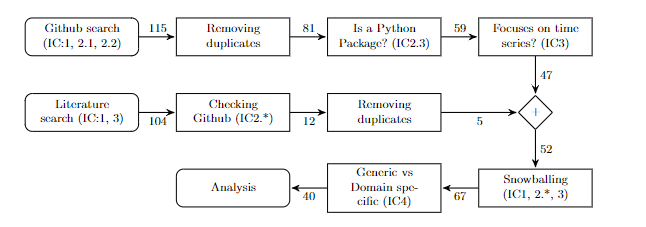
\includegraphics[width = 14cm]{Figures/metodologia.png } 
    \caption{Busqueda y filtrado de procesos, las etiquetas de las flechas indican el número de repositorios discriminados tras cada paso.}
    \label{Fig. 01}     
\end{figure}

\subsection{Preguntas de investigación}

Se formaliza la meta del articulo.  La idea es \textbf{análizar} las paquetereias de Python dedicadas a análisis de series de tiempo con el propósito de estructurar las implementaciones disponibles con respecto a las implementaciones desde el punto de vista del practicante. Los cuestionamientos son:
\begin{enumerate}
    \item ?`Cuáles cometidos para análisis de series temporales existen? y ?`Cuáles de estas implementaciones están en alguna paquetería de Python?
    \item ?`Cómo las paqueterías apoyan la evaluación del resultado producido?
    \item ?`Cómo las paqueterías apoyan su uso, que percepción se dá para estimar la duración de dichas paquetereias ?
\end{enumerate}

\subsection{Criterio de inclusión}

Para guiar la revición y filtración de las paqueterías reelvantes, los autores definieron los siguientes críterios de  inclusión. El paquete debe ser de dominio público, escrito en Python, y disponible en GitHub. El paquete debe ser estar bajo activo mantenimiento. Debe tener más de 100 estrellas de GitHub. Debe estar listado el el PyPI (Python Package Index, un repositorio de software). Se debe poder instalar via pip o conda. El paquete explicitamente debe enfocarse en análisis de series temporales. Finalmente, se excluyen paqueterías que se enfocan en series de tiempo para un campo en partícular, como finanzas, ciencias de la tierra, audio, etc.

\subsection{Buscando repositorios de dominio público en GitHub}

El articulo nos menciona que filtraron los repositories de GitHub por lenguaje (Python), número de estrellas, y aquellos repositorios que se hayan actualizado después de Julio del 2020.

Con la finalidad de seleccionar una lista de temas reelevantes, manualmente se seleccionó una \textbf{lista de ocho paqueterías} de Python conocidas para ser usadas en análisis de series temporales: pandas, numpy, scipy, statsmodel, ruptures, tsfresh, tslearn, and sktime. Se examinaron los temas usados en cada paquetería. En total se consideran 16 funciones o temas diferentes. De los 115 repositorios encontrados en GitHub, tras el proceso de inclusión-discriminación ilustrado en Fig.\ref{Fig. 01}, se llegó a que solo 40 repositorios son candidatos a examinar.

\subsection{Buscando bases de datos en bibliografía cientifica}

La busqueda de paqueterias solo en un repositorios podira no ser suficiente para cubrir todas las paqueterías existentes. Como por ejemplo fue el caso de la paquetería tsfresh. Los autores usaron basesd de datos como IEEE Xplore, ACM Digital Library, Web od Science, Scopus y Journal of Opne Source Software (JOSS)  , Zenodo.  Por ejemplo, para las primeras cuatro, usaron un query para filtrar dichas paqueterías. Se encontró que cinco de estos repositorios no se encontraban en GitHub, estas fueron: tsfreash, neurodsp, EoN, nolds, y pastas.

\subsection{Snowballing}

Con el propósito de extender la investigación, se usó una acercamiento \textit{snowballing}. Manualmente, los autores revizarion cada paquetería para encontrar link a otras librerias. De igual forma, manualmente se revisó la documentación y los repositorios de GitHub para ver si incluian trabajos relacionados. 15 nuevas paqueterías se incluyeron en el análisis despues de lo anteriormente descrito. 

\subsection{Genérico vs dominio específico}

Como ya se hablo antes, se seleccionaron los paqutes que no se enfucan en una disciplina en partícular que no sea anális de series temporales.


\section{Resultados}

\subsection{Implementación de cometidos para análisis de series temporales}

Para contestar la primer pregunta de investigación, primeramente se revizarion los cometidos presentes en la literatura y luego se analizaron en cada uno de los 40 paquetes clasificando cual es capaz de procesar dicho cometido.

Definición de los cometidos
\begin{enumerate}
    \item \textbf{Indexing: } Dada una serie de tiempo y algunas similitudes de medida, encuentra la serie de tiempo más cercana.
    \begin{figure}[H] 
        \centering 
        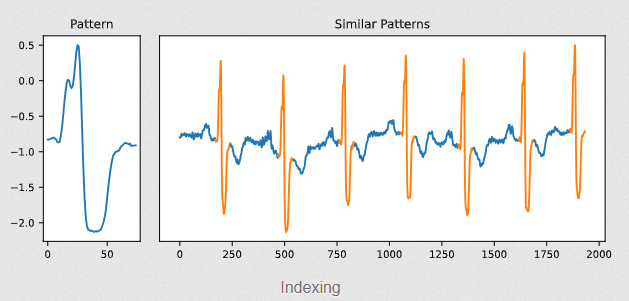
\includegraphics[width = 10 cm]{Figures/T8.png} 
        % \caption{}
        \label{Fig. 1}
    \end{figure} 
    \item \textbf{clustering: } Encuentra grupos de series temporales similares.
    \begin{figure}[H] 
        \centering 
        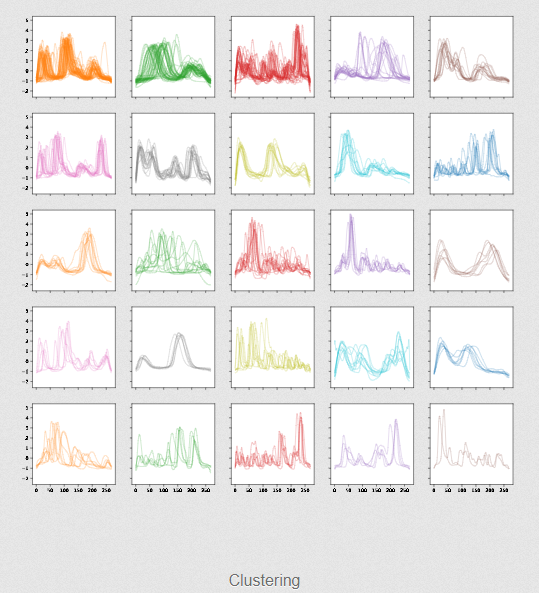
\includegraphics[width = 10 cm]{Figures/T3.png} 
        % \caption{}      
        \label{Fig. 2}
    \end{figure} 
    \item \textbf{clasificación: } Asigna a cada serie temportal una clase predefinida.
    \begin{figure}[H] 
        \centering 
        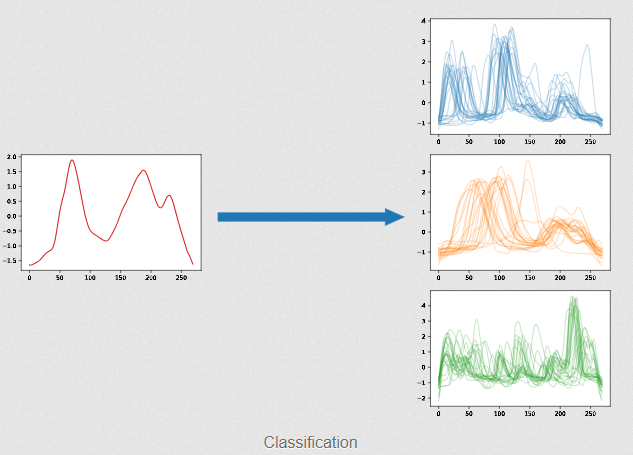
\includegraphics[width = 10 cm]{Figures/T2.png } 
        % \caption{}
        \label{Fig. 3}
    \end{figure} 
    \item \textbf{Segmentación: } Crea una aproximación precisa de una serie temporal por reducción de su dimensión mientras retiene carácteristicas especiales.
    \begin{figure}[H] 
        \centering 
        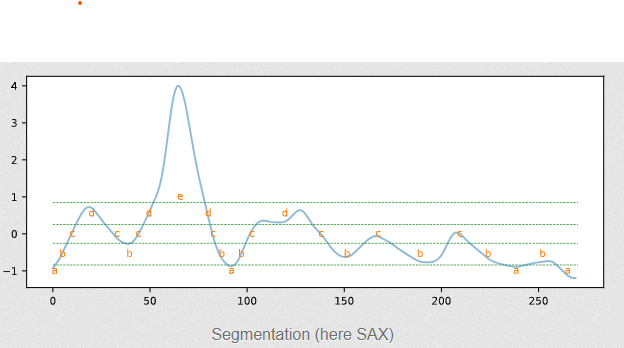
\includegraphics[width = 10 cm ]{Figures/T5.png} 
        % \caption{}
        \label{Fig. 4}
    \end{figure} 
    \item \textbf{Pronóstico: } Dada una serie de tiempo hasta un tiempo $t_n$, pronósticar los siguientes valores.
    \begin{figure}[H] 
        \centering 
        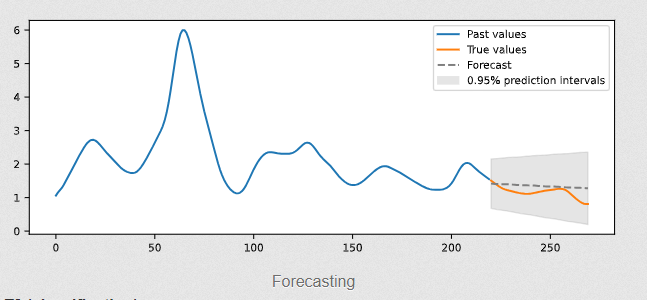
\includegraphics[width = 10 cm]{Figures/T1.png} 
        % \caption{}
        \label{Fig. 5 }
    \end{figure} 
    \item \textbf{Detección de anomalias: } Encuentra subsecuencias de la serie de tiempo, también llamadas discords.
    \begin{figure}[H] 
        \centering 
        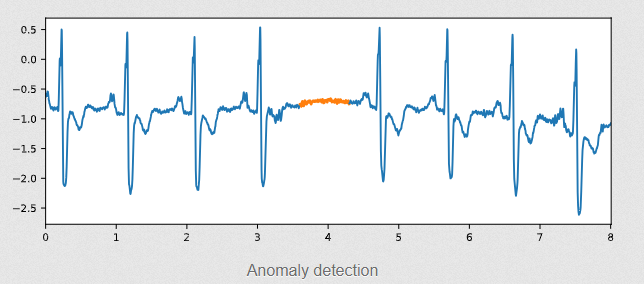
\includegraphics[width =10 cm ]{Figures/T4.png} 
        % \caption{}
        \label{Fig. 6}
    \end{figure} 
    \item \textbf{Motif Discovery: } Encuentra cada suvsecuencia (llamada Motif) que parece governar la serie temporal recurrentemente.
    \begin{figure}[H] 
        \centering 
        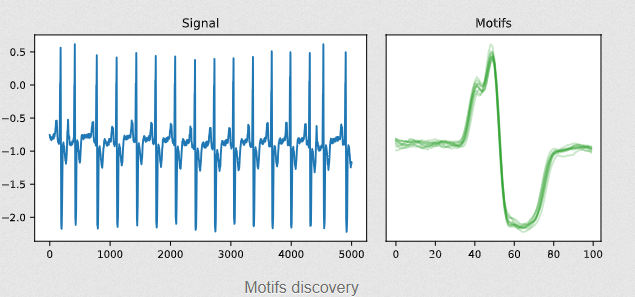
\includegraphics[width = 10 cm ]{Figures/T6.png} 
        % \caption{}
        \label{Fig. 7}
    \end{figure} 
    \item \textbf{Rules Discovery: } Encuentra las reglas que podrían governar la asociación entre conjuntos de subsecuencias de series temporales.
    % \begin{figure}[H] 
    %     \centering 
    %     \includegraphics[width = ]{Figures/} 
    %     \caption{}
    %     \label{Fig. }
    % \end{figure} 
\end{enumerate}

Tambien definen los compnentes para la Implementación
\begin{enumerate}
    \item \textbf{Preprocesamiento: } Filtración de ruido, remover valores atípicos, imputación de valores faltantes.
    \item \textbf{Representación: } Reducción de dimensionalidad, encontrar formas carácteristicas fundamentales.
    \item \textbf{Medidas de semejanza:}
    \item \textbf{Esquemas de identación:}
\end{enumerate}

\textbf{Cometidos implementados} Se encontró que las paqueterías explicitamente mencionan los cometidos correspondientes al de la literatura. Se encontró que 6 paquetes prooven de pronosticos, 6 paquetes prooven clasificación, 6 prooven metodos de clustering, 6 prooven detección de anomalias, y 4 prooven métodos de segmentación; 4 que prooven reconocimiento de patrones; y abarcando la identación con motif Discovery en una categoria, hay cinco paquetes que prooven dichos cometidos.

Luego, para las implementacionesd de componentes, se encontro que 4 paquetes ecplicitamente prooven reducción de dimensionalidad, 17 paquetes prooven imputación de valores faltantes,24 paquetes prooven métodos de transformación y generación de carácteristicas. y 7 paquetes prooven vétodos para computar medidades de similaridad. La tabla 4 en el articulo resume cual paquete es capaz de ciertos cometidos.

\subsection{Uso de paquetes y comunidades}

Para responder a la tercer pregunta de investigación, se extrajo información acercad e la documentación, las dependencias, y la comunidad que apoya dichos paquetes. Por ejmple, GitHub proove de varios repositorios de estadística que puede ser usados para optener una idea de la esperanza de vida de lso paquetes. Se usó el numero de estrellas de GitHub y los \textit{forks} para estimar la comunidad detras de cada paquete. Las siguiente figura ilustra la cantidad de de estrellas y \textit{forks} para estimar la comunidad.

\begin{figure}[H] 
    \centering 
    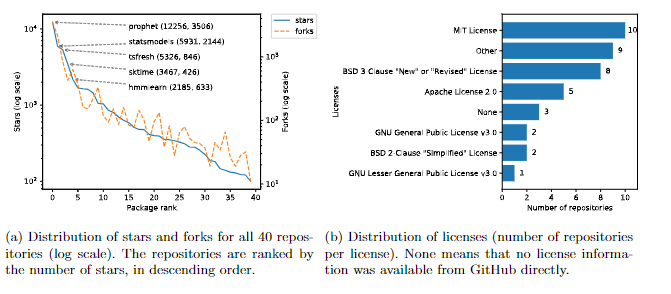
\includegraphics[width = 16 cm ]{Figures/stars.png } 
    % \caption{}
    \label{Fig. 02}
\end{figure} 

Casi todos los paqutes depende en numpy. Las paquetes con mayor dependencia son numpy, scipy, pandas, scikit-learn, y matplotlib.



\section{Discusión y amenazas para la validación}

En esta sección se discuten las elecciones que hicieron los autores que puedan afectar la validiación del articulo. Esta revisión se centra en GitHub. Se limitaron a repositorios con al menos 100 estrellas. Esto es algo arbitrario sobre todo para paquetes con cerca de 100 estrellas.

Varios paquetes no pudieron ser encontrados de forma automatica. Por ejemplo, el paquete cesium no lista en GitHub, sino que fue encontrado tras el \textit{snowballing}. Trataron de automatizar algunos de los cometidos, usando PyPI y la API de GitHub, o la herramienta johnnydep. Hubo varios falsos positivos. Por lo que fue necesario checar cada uno manualmente.
De igual forma, saber si un paquete se concentra en un dominio especifico es algo ambiguo o difuso, entonces decidieron tomar un acercamiento conservativo para mantener la revisión concentrada en series temporales.

La clasificación de los paquetes está en la tabla 4 del articulo, que vemos en la siguiente figura
\begin{figure}[H] 
    \centering 
    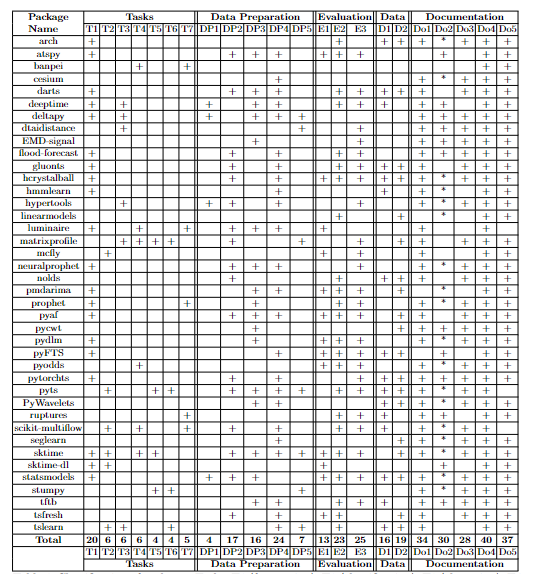
\includegraphics[width = 14cm]{Figures/packages.png} 
    \caption{Clasificación de paqueterías. Tasks: T1(Pronóstico),T2 (clasificación), T3 (clustering), T4 (detección de anomalias), T5 (Segmentación), T6 (reconocimiento de patrones), T7(Cambio del putn de detección). Preparación de los datos(componentes de implementación): DP1 (reducción de dimensionalidad), DP2 (imputación de valor ausente), DP3 (descomposición), DP4 (preprocesamiento), DP5 (medidas de similaridad). Evaluaciones: E1 (selección de modelos, busqueda hiperparámetrica, selección de carácteristicas), E2 (metricas y pruebas estadísticas), E3 (visualización). Bases de datos: D1 generación sintética de datos, D2 (continen bases de datos). Documentación: Do1 (documentación dedicada), Do2 (notebook ejecutable), Do3 (referecia API), Do4 (guia de instalación), Do5 (guia al usuario).}
    \label{Fig. }
\end{figure} 


\section{Conclusión}

En el articulo se presentó una revisión sistematica de 40 paqueterías de Python dedicadas a series temporales. Los autores propusieron una categorización de los paquetes según el análisis implementado. Tambien discutieron el procediemento de busqueda de tales paqueterías, los posibles sesgos y retos encontrados mientras se hacia dicha actividad. Como los paquetes iran evolucionando, los autores mantienen una lista actualizada en su pagina de GitHub en \textit{https://siebert-julien.github.io/time-series-analysis-python/overview.html}.


% \bibliographystyle{plain} % We choose the "plain" reference style
% \bibliography{refs} % Entries are in the refs.bib file

% \cite{Brockwell}

\begin{thebibliography}{9}

  \bibitem{Siebert}
  Siebert, J., Groß, J., and Schroth, C. (2021). A systematic review of python packages for time series analysis. arXiv preprint arXiv:2104.07406.

  \bibitem{Brockwell}
  Brockwell, P. J., and Davis, R. A. (Eds.). (2002). Introduction to time series and forecasting. New York, NY: Springer New York.
  
  
  \end{thebibliography}





















\end{document}